\documentclass{mwart}
\usepackage[utf8]{inputenc}
\usepackage{indentfirst}
\usepackage{polski}
\usepackage{float}
\usepackage{hyperref}
\usepackage{amsmath}
\usepackage{xcolor}
\usepackage{listings}
\usepackage[caption = false]{subfig}
\usepackage[final]{graphicx}
\usepackage[a4paper, total={6in, 8in}]{geometry}

\usepackage{xcolor}
\usepackage{listings}
\usepackage{longtable}
\usepackage{natbib}
\usepackage{graphicx}

\definecolor{mGreen}{rgb}{0,0.6,0}
\definecolor{mGray}{rgb}{0.5,0.5,0.5}
\definecolor{mPurple}{rgb}{0.58,0,0.82}
\definecolor{backgroundColour}{rgb}{0.95,0.95,0.92}
\lstdefinestyle{JavaStyle}{
    backgroundcolor=\color{backgroundColour},   
    commentstyle=\color{mGreen},
    keywordstyle=\color{magenta},
    numberstyle=\tiny\color{mGray},
    stringstyle=\color{mPurple},
    basicstyle=\footnotesize,
    breakatwhitespace=false,         
    breaklines=true,                 
    captionpos=b,                    
    keepspaces=true,                 
    numbers=left,                    
    numbersep=5pt,                  
    showspaces=false,                
    showstringspaces=false,
    showtabs=false,                  
    tabsize=2,
    language=Java
}

\title{
    \textbf{Algorytmy ewolucyjne i metaheurystyki}\\ 
    \begin{large} 
        Sprawozdanie 1
    \end{large}
}

\author{
    Górka Bartosz\\
  \texttt{127228}
  \and
  Zimniak Kajetan\\
  \texttt{127229}
}

\date{}
\begin{document}

\maketitle

\section{Opis problemu}
Celem projektu było przygotowanie dwóch wersji algorytmów rozwiązujących problem grupowania. Liczba grup została ustalona na $10$. Funkcja celu to minimalizacja średniej odległości wszystkich par obiektów umieszczonych w ramach tej samej grupy.

Jako kluczowe było wykorzystanie macierzy odległości (dystansu pomiędzy punktami) zamiast użycia przestrzeni kartezjańskiej jako punktu wyjścia. Takie założenie pozwala wykorzystać algorytmy również w przypadku zmiany funkcji odległości (macierz odległości jest wystarczająca do dokonania przydziału).

\section{Pseudokody przygotowanych algorytmów}
\subsection{Algorytm zachłanny}
Algorytm zachłanny dokonuje przydziału obiektu zgodnie z pseudokodem zaprezentowanym poniżej. Dla każdego punktu wybiera grupę do której ma najmniejszą wartość odległości (pomiędzy obecnym punktem a punktem startowym grupy). Po wybraniu najlepszego przydziału (najmniejsza odległość), dodajemy punkt do listy punktów przynależących do wybranej grupy. Inicjalizacja punktów startowych odbywa się poprzez losowy wybór elementu startowego w każdej z grup.

\begin{lstlisting}[style=JavaStyle]
for each point in list of points {
    int pointID = point.getPointID();
    int selectedGroupID;
    double minDistance = Double.Max_Value;

    for each groupIndex in groups groups {
        double distance = distanceMatrix[groupIndex][pointID];
        
        if (distance < minDistance) {
            minDistance = distance;
            selectedGroupID = groupIndex;
        }
    }

    pointsInGroup[selectedGroupID].add(point);
}
\end{lstlisting}

\subsection{Algorytm z wykorzystaniem żalu}
Algorytm z wykorzystaniem żalu dokonuje przydziału obiektu zgodnie z pseudokodem zaprezentowanym poniżej. W każdej iteracji przydziela jeden punkt do jednej grupy. Dla każdego punktu sprawdza jak bardzo jego dołożenie do danej grupy pogorszy wartość funkcji celu. Następnie wybiera punkt, którego dołożenie do którejś z grup będzie najmniej korzystne i dołącza go do grupy, która znajduje się najbliżej niego (najkorzystniejszy wybór wśród wszystkich grup). Inicjalizacja punktów startowych odbywa się poprzez losowy wybór elementu startowego w każdej z grup.

\begin{lstlisting}[style=JavaStyle]
pointsInGroup = []
while notAlreadyUsedPointsList not empty:
    objectiveValuesForPointsList = [][]
    for each point in list of points:
        for each group in groups:
            //calculate mean of distances between all pair of points in this group
            objectiveValuesForPointsList[group][point] =
                calculateMeanOfDistancesInGroup(group)
    chosenGroup, chosenPoint =
        chooseBiggestObjectiveAndReturnBestGroup(objectiveValuesForPointsList)
    pointsInGroup[chosenGroup].add(chosenPoint)
        
\end{lstlisting}

\section{Wyniki eksperymentów obliczeniowych}
W tabeli \ref{table:wyniki} zaprezentowano wyniki eksperymentów obliczeniowych. Dokonano $100$ powtórzeń obliczeń, za każdym razem z losowym wyborem elementu startowego w każdej z $10$ grup. Obydwa algorytmy wykorzystywały te same punkty startowe w ramach pojedynczej iteracji.

\begin{table}[H]
\centering
\caption{Wyniki eksperymentów obliczeniowych dla 100 iteracji}
\label{table:wyniki}
\resizebox{\textwidth}{!}{%
\begin{tabular}{|c|r|r|}
\hline
\textbf{Cecha}                                                                     & \multicolumn{1}{c|}{\textbf{Algorytm zachłanny}} & \multicolumn{1}{c|}{\textbf{Algorytm oparty o żal}} \\ \hline
\textbf{\begin{tabular}[c]{@{}c@{}}Wartość minimalna\\ funkcji celu\end{tabular}}  
&   33.92                                               
&   37.62                                                 \\ \hline
\textbf{\begin{tabular}[c]{@{}c@{}}Wartość maksymalna\\ funkcji celu\end{tabular}} 
&   44.44                                              
&   73.82                                                 \\ \hline
\textbf{\begin{tabular}[c]{@{}c@{}}Wartość średnia\\ funkcji celu\end{tabular}}    
&   38.47                                               
&   48.36                                                  \\ \hline
\textbf{\begin{tabular}[c]{@{}c@{}}Wartość minimalna\\ czasu obliczeń {[}sec{]}\end{tabular}} 
&   0,000804                                               
&   0,18                                                  \\ \hline
\textbf{\begin{tabular}[c]{@{}c@{}}Wartość maksymalna\\ czasu obliczeń {[}sec{]}\end{tabular}} 
&   0,029                                               
&   1,52                                                  \\ \hline
\textbf{\begin{tabular}[c]{@{}c@{}}Wartość średnia\\ czasu obliczeń {[}sec{]}\end{tabular}} 
&   0,0017                                               
&   0,258                                                  \\ \hline
\end{tabular}%
}
\end{table}



\section{Wizualizacja najlepszych rozwiązań}
\subsection{Algorytm zachłanny}
\begin{figure}[H]
    \centering
    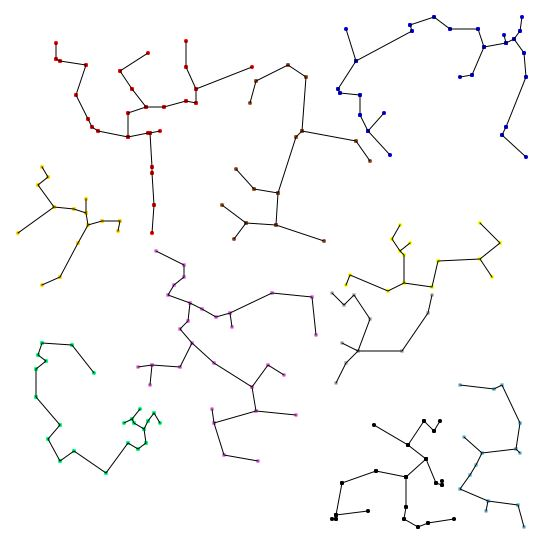
\includegraphics[width=\textwidth]{zachlanny2.png}
    \caption{Algorytm zachłanny - wizualizacja najlepszego przydziału}
\end{figure}

\subsection{Algorytm oparty o żal}
\begin{figure}[H]
    \centering
    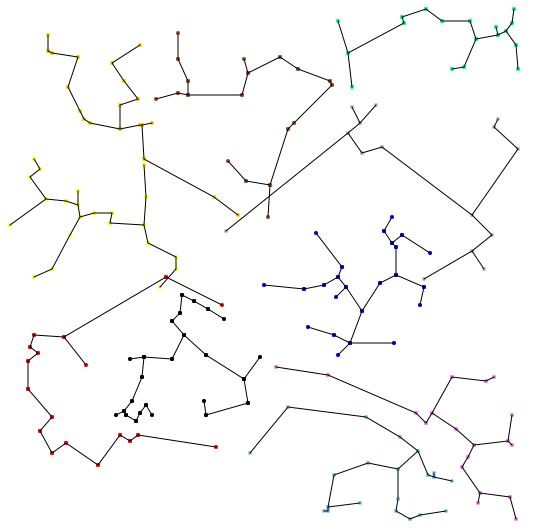
\includegraphics[width=\textwidth]{regret2.png}
    \caption{Algorytm oparty o żal - wizualizacja najlepszego przydziału}
\end{figure}

\end{document}
